%=================================================================
% fp-tools BioMedInformatics manuscript
% Compile with: latexmk -pdf main.tex   (or pdflatex x3)
% Requires the MDPI class shipped under Definitions/ (extracted from
% manuscript/templates/MDPI_template_ACS.zip by manuscript/scripts/prepare_biomedinformatics_template.py)
%=================================================================
\documentclass[biomedinformatics,article,submit,pdftex,moreauthors]{Definitions/mdpi}

% MDPI internal commands - do not modify
\firstpage{1}
\makeatletter
\setcounter{page}{\@firstpage}
\makeatother
\pubvolume{1}
\issuenum{1}
\articlenumber{0}
\pubyear{2026}
\copyrightyear{2026}
\datereceived{ }
\dateaccepted{ }
\datepublished{ }

%------------------------------------------------------------------
\Title{fp-tools: A Reproducible Platform for ATAC-seq Footprinting and
Regulatory Motif Analysis}

\Author{Yaoxiang Li $^{1}$ and Chunling Yi $^{1,}$*}

\AuthorNames{Yaoxiang Li and Chunling Yi}

\address{%
$^{1}$ \quad Department of Oncology, Lombardi Comprehensive Cancer Center, Georgetown University Medical Center, Georgetown University, Washington, DC, USA; yl814@georgetown.edu (Y.L.); cy232@georgetown.edu (C.Y.)}

\corres{Correspondence: cy232@georgetown.edu (C.Y.)}

\abstract{ATAC-seq footprinting enables near-base-resolution inference of
transcription-factor (TF) occupancy across the genome. However, the field lacks a
computationally efficient, user-friendly, and integrated platform that accepts
both bulk and single-cell ATAC-seq data, supports both de novo motif discovery
and matching to public motif databases, and generates interactive and
publication-ready visual outputs. Here, we present \texttt{fp-tools}, a Python
package that builds on the widely used ATAC-seq footprinting framework TOBIAS.
We substantially improve computational efficiency across key steps, including Tn5
bias correction, footprint calling, and motif matching. In addition,
\texttt{fp-tools} introduces de novo motif discovery, replicate-aware
differential footprinting, and scaled motif aggregation, all features not
provided by TOBIAS. We further streamline a single-cell ATAC-seq footprinting
workflow, provide interactive visualization of analysis results, and implement a
graphical user interface (GUI) that enables code-free execution of all package
commands. Using public bulk ATAC-seq replicates and single-cell datasets, we
demonstrate that \texttt{fp-tools} quantitatively recovers cell-type-specific
TF-binding patterns and identifies de novo binding motifs that are not captured
by existing public motif databases. Together, \texttt{fp-tools} provides a
highly efficient, accessible, and comprehensive platform for TF footprint
analysis across bulk and single-cell ATAC-seq studies.}

\keyword{ATAC-seq; transcription factor footprinting; chromatin accessibility;
motif analysis; replicate-aware differential footprinting; de novo motif
discovery}

% Use an external BibTeX database (references.bib) with the MDPI style.
\externalbibliography{yes}

\begin{document}

%==================================================================
\section{Introduction}
%==================================================================

Assay for Transposase-Accessible Chromatin using Sequencing (ATAC-seq) has
become a standard tool in epigenetic and transcriptional studies~\cite{buenrostro2013}.
By using a hyperactive Tn5 transposase to insert sequencing adapters into
accessible regions of DNA, ATAC-seq enables rapid and sensitive identification
of regulatory elements such as promoters, enhancers, and insulators. With the
development of single-cell ATAC-seq (scATAC-seq), this approach has further
enabled the characterization of cell-type-specific regulatory programs within
complex tissues~\cite{buenrostro2015scatac}.

Less widely recognized is that deeper analysis of the local depletion of Tn5 cut
sites within accessible chromatin can reveal transcription factor (TF) occupancy
at near base-pair resolution, producing characteristic protected regions known as
``footprints.'' Compared with standard motif enrichment analysis, which evaluates
only the frequencies of TF motifs within accessible regions, footprinting
provides more direct evidence of TF binding and quantitative information about
binding strength by measuring the difference in accessibility between the
protected footprint center and its flanking regions. However, the requirement for
additional computational processing, careful correction for Tn5 insertion bias,
and specialized analytical tools has limited its broader adoption.

Earlier footprinting methods, including CENTIPEDE, Wellington, PIQ, DeFCoM, and
HINT, established important frameworks for detecting TF occupancy from chromatin
accessibility data~\cite{pique2011centipede,piper2013wellington,sherwood2014piq,quach2017defcom,li2019hint}.
Several of these methods were developed primarily around DNase-seq and did not
directly address the strong sequence preferences of Tn5 transposase in ATAC-seq.
HINT-ATAC incorporated Tn5 bias into footprint detection by modeling
position-dependent cleavage patterns~\cite{li2019hint}, whereas TOBIAS further
refined Tn5 correction by first estimating expected insertion bias from local
sequence context and adjusting the observed cut-site signal before footprint
scoring~\cite{bentsen2020}. This explicit correction reduces the likelihood that
sequence-driven Tn5 insertion preferences are misinterpreted as TF-associated
protection, thereby improving the reliability of ATAC-seq footprint inference.

More recently, PRINT/scPrinter, maxATAC, and ChromBPNet have advanced
ATAC-seq-based TF binding inference through multiscale footprinting and
deep-learning models~\cite{hu2024print,cazares2023maxatac,chrombpnet2024}.
Although powerful, these approaches remain challenging for broad adoption by
experimental researchers because they often require complex software setup,
large training or reference datasets, GPU-oriented computation, or less
transparent model interpretation. In contrast, TOBIAS provides a more accessible
ATAC-seq footprinting framework with explicit Tn5 bias correction and
interpretable footprint scores~\cite{bentsen2020}. However, TOBIAS remains
primarily command-line based and does not natively support de novo motif
discovery, replicate-aware statistics, or streamlined single-cell ATAC-seq
footprinting workflows.

We developed \texttt{fp-tools} to address these unmet needs. The package
preserves the interpretable, motif-centered footprinting logic of TOBIAS while
improving the speed, usability, and scope of the core analysis. Compared with
TOBIAS, \texttt{fp-tools} adds de novo motif discovery with database matching,
replicate-aware differential footprint analysis, scaled motif aggregation,
streamlined single-cell ATAC-seq footprinting, interactive HTML reports, editable
SVG outputs, and a graphical user interface (GUI) for code-free execution of
command-compatible workflows.

By connecting common TF-footprinting tasks into a unified, auditable workflow
that can be run from the command line, saved YAML configuration files, or the
GUI, \texttt{fp-tools} makes footprinting more accessible to both computational
and experimental researchers. Here, we describe the implementation of
\texttt{fp-tools} and evaluate its performance using public bulk ATAC-seq
replicate datasets and single-cell ATAC-seq datasets, demonstrating its potential
to expand the routine use of footprinting in regulatory genomics studies.


%==================================================================
\section{Materials and Methods}
%==================================================================

\subsection{Core Signal Model and Footprint Scoring}

\texttt{fp-tools} uses a command-oriented workflow in which corrected cut-site
tracks, genomic regions, motif annotations, sample labels, and output files
follow consistent conventions. This allows bias-correction outputs to be used
directly for footprint scoring, motif-anchored differential analysis, and
aggregate visualization around transcription factor binding sites (TFBSs) or
user-defined genomic regions. YAML configuration files record input files and
analysis parameters so the same workflow can be rerun without modifying the
underlying methods.

Following the signal model popularized by TOBIAS~\cite{bentsen2020},
\texttt{fp-tools} treats base-resolution, bias-corrected Tn5 cut-site profiles
as the primary signal for footprint analysis. This design preserves the standard
bulk ATAC-seq footprinting interpretation, in which putative TF occupancy is
inferred from a local depletion of corrected cut sites at a motif or candidate
binding site relative to the surrounding accessible flanks. Bias correction
estimates the sequence-driven component of Tn5 insertion and produces corrected
cut-site tracks in which local depletion and enrichment are less likely to
reflect transposase sequence preference alone. After bias correction,
\texttt{fp-tools} can optionally rescale corrected cut-site tracks before
footprint scoring. When this option is enabled, a single multiplicative scale
factor is estimated for each sample from shared background regions. If
$q_{s,0.95}$ denotes the 95th percentile of corrected signal for sample $s$ over
the shared background regions and $\tilde{q}_{0.95}$ denotes the across-sample
target, typically the median of the sample-level 95th percentiles, the rescaled
signal is
\[
x'_{s,i}=x_{s,i}\frac{\tilde{q}_{0.95}}{q_{s,0.95}} .
\]
This robust q95 scaling reduces sample-to-sample differences in overall signal
magnitude while preserving the shape of each sample's corrected signal profile,
without forcing the complete empirical signal distributions to be identical.

For footprint scoring, let $x_i$ denote the corrected Tn5 cut-site signal at
position $i$ around a candidate footprint position $p$, after optional q95
scaling when enabled. The default footprint score is calculated as a
center-versus-flank contrast,
\[
F(p)=\frac{1}{|L|+|R|}\left(\sum_{i\in L}x_i+\sum_{i\in R}x_i\right)-
\frac{1}{|C|}\sum_{i\in C}x_i,
\]
where $C$ denotes the protected center window and $L$ and $R$ denote the left
and right flanking windows. Window sizes are user-configurable and are recorded
with the analysis parameters. Larger values indicate lower corrected cut-site
signal in the center than in the surrounding flanks, corresponding to the
expected footprint pattern of reduced Tn5 cleavage at a putative bound site and
higher cleavage in nearby accessible DNA.


\subsection{Known-motif Scanning and Motif-site Definition}

For motif-anchored footprint analysis, \texttt{fp-tools} scans candidate
accessible regions for transcription factor motif matches using position weight
matrices from a user-supplied motif database, such as JASPAR 2026 CORE
vertebrates non-redundant motifs~\cite{jaspar2026}. The GC content of the
accessible-region sequence set is used as the background nucleotide distribution
for log-odds motif scoring, and motif-specific score thresholds are derived from
the configured motif-match p-value cutoff. Both strands are scanned. For each
motif, overlapping candidate matches for that motif are resolved by retaining
the higher-scoring match, so each motif contributes a non-overlapping site set
for downstream analysis.

Each motif site is represented by its genomic interval, motif identifier, strand,
motif score, associated peak or region annotation, and the footprint score
measured from each input signal track. For motif $m$, let $S_m$ denote the
candidate sites assigned to that motif within the common accessible-region
universe. Background positions $B$ are sampled from the same accessible-region
universe and are used to estimate the expected distribution of footprint-score
changes not specifically associated with scanned motif sites. This shared
motif-site and background-position representation allows single-sample,
replicate-supported, and de novo-augmented analyses to use the same downstream
differential footprinting framework.

When de novo motifs are discovered and matched to known motifs, the discovered
motif set can be analyzed independently or appended to the known motif database
and scanned using the same motif-site conventions.


\subsection{De Novo Motif Discovery}

The de novo motif discovery module begins from candidate footprint intervals,
which may be produced by footprint calling or provided as input. For each
candidate interval $j$ with center $p_j$, BED-like strand annotation $a_j$, and
flank size $h$, it extracts a candidate-centered sequence from the reference
genome. Using one-based inclusive notation for clarity, this sequence has length
$2h+1$ and is written as
\[
S_j =
\begin{cases}
G[p_j-h,\,p_j+h], & a_j \in \{\texttt{+}, \texttt{.}\},\\
\mathrm{revcomp}\{G[p_j-h,\,p_j+h]\}, & a_j = \texttt{-}.
\end{cases}
\]
Thus, positive-strand and unstranded candidate intervals are exported in the
reference-genome orientation, whereas negative-strand intervals are
reverse-complemented before motif discovery.
When half-open BED-style coordinates are used internally, interval endpoints are
converted before sequence extraction so that the exported FASTA sequence remains
centered on $p_j$. The module records the input intervals, genome build, flank
width, software versions, and the parameters passed to MEME, DREME, or
STREME~\cite{bailey2015meme,Bailey2011_DREME,Bailey2021_STREME} for motif
discovery. When database comparison is requested, the corresponding
Tomtom~\cite{gupta2007tomtom} settings are also recorded. STREME was designed
for accurate motif discovery from enriched sequence sets~\cite{Bailey2021_STREME}.
Discovered motifs can be analyzed as an independent motif set or matched to a
known database such as JASPAR 2026~\cite{jaspar2026} and appended to the known
motif set for downstream differential footprint analysis. In this design,
candidate FASTA export, motif discovery, motif comparison, and database
augmentation become part of the recorded footprint analysis.

\subsection{Pseudobulk Fragment Aggregation}

The pseudobulk module groups single-cell ATAC fragments by a metadata column,
such as cell type, cluster, donor, or treatment. Let $F_b$ be the multiset of
fragments assigned to barcode $b$, and let $g(b)$ be its group label. The
pseudobulk fragment collection for group $k$ is the concatenated multiset
\[
F_k = \mathrm{concat}_{b:g(b)=k}(F_b),
\]
so repeated fragments and fragment multiplicity are preserved. Thus, the
pseudobulk profile represents the sum of fragments from cells assigned to a
group, rather than a binarized representation of accessible regions. Groups that
pass specified cell-count and fragment-count filters are written as bulk-like
fragment files with manifest records. When genome sizes are supplied,
\texttt{fp-tools} can also emit counts per million cut sites (CPM)-normalized
cut-site bigWigs,
\[
y_{k,t}=10^6\frac{c_{k,t}}{\sum_u c_{k,u}},
\]
where $c_{k,t}$ is the cut-site count for group $k$ at genomic position $t$. These
tracks support motif-centered aggregate profiles matched to the bulk ATAC-seq
analysis path. The full pseudobulk route writes pseudo-paired BAMs from grouped
fragment endpoints and then runs correction, scoring, motif-aware comparison, and
plotting with the same conventions used for bulk ATAC-seq.

\subsection{Cell-level Footprint-signature Visualization}

For cell-level marker visualization, \texttt{fp-tools} computes
K-nearest-neighbor (KNN)-smoothed footprint signatures from single-cell fragments.
For each marker TF, motif centers are scanned inside the selected accessible-bin
universe. Fragment cut sites are counted in a $\pm$100 bp window around those
motif centers for each barcode. Each cell is assigned a local neighborhood
profile by summing cut-site profiles across its 75 nearest neighbors in the
single-cell embedding, and a flank-minus-center footprint-signature score is
computed from that neighborhood profile. Marker TFs are selected from the
pseudobulk differential-footprint results and biological prior marker sets before
display orientation is applied. For visualization only, signatures are oriented
so that higher values correspond to the marker-associated cell population and are
then standardized per TF for UMAP display. These KNN-smoothed signatures are
used for cell-level visualization of motif-centered cut-site patterns, whereas
full bias-corrected footprint tracks and statistical comparisons are computed
from grouped pseudobulk profiles.

\subsection{Replicate-aware Differential Footprint Analysis}
\label{sec:replicate}

The differential footprint module supports both single-sample contrasts and
replicate-supported comparisons. It retains conventional motif-centered
footprint-score logic while adding repeated condition labels, replicate-level
summaries, and replicate-aware testing.
Repeated condition names, such as \texttt{--cond-names Bcell Bcell Tcell
Tcell}, define biological replicate groups while preserving the original
differential-footprint output structure. Let $x_{c,r,i}$ be the footprint score
at site or background position $i$ for replicate $r$ of condition $c$.

For single-sample versus single-sample contrasts, \texttt{diff-footprints} uses
the motif-site versus background-distribution comparison of the standard
TOBIAS-style report. Candidate sites are grouped by motif, site-level changes at
motif sites are compared with changes at sampled background positions, and
p-values are adjusted across motifs within each contrast.

For replicate-supported comparisons, \texttt{fp-tools} generalizes this
comparison to multiple samples per condition. Footprint scores are computed for
each replicate on the same peak and motif-site universe. Replicate scores are
then summarized within each condition,
\[
\bar{x}_{c,i}=\frac{1}{n_c}\sum_{r=1}^{n_c}x_{c,r,i},
\qquad
s^2_{c,i}=\frac{1}{n_c-1}\sum_{r=1}^{n_c}(x_{c,r,i}-\bar{x}_{c,i})^2 .
\]
For motif $m$, let $S_m$ denote its candidate motif sites and let $B$ denote the
sampled background positions from the same accessible-region universe. The
replicate-aware motif-background effect is reported as
\[
\Delta_m =
\frac{1}{|S_m|}\sum_{i\in S_m}(\bar{x}_{c_1,i}-\bar{x}_{c_2,i})
-
\frac{1}{|B|}\sum_{i\in B}(\bar{x}_{c_1,i}-\bar{x}_{c_2,i}) .
\]
The report also includes replicate counts, condition means, SDs, and SE
summaries, so the additional samples contribute to a more stable estimate rather
than being collapsed outside the analysis.

Quantile-based score scaling remains an optional comparison-stage adjustment. In
single-sample contrasts, sample-level quantile scaling provides the conventional
two-sample score-distribution matching. In replicate-supported comparisons,
condition-level background quantile scaling fits a quantile-based normalization
curve from positive background-score quantiles for each condition and applies the
corresponding condition curve before condition summaries are computed. This
option is used as a sensitivity adjustment; the main replicate-aware extension is
the explicit use of replicate-level motif scores.

When per-sample motif-score matrices are available, \texttt{fp-tools} further
applies empirical-Bayes variance moderation across motifs, following the
moderated testing framework of Smyth~\cite{smyth2004}. This
replicate-supported matrix view estimates condition effects from per-sample
motif-site scores and is reported alongside, rather than replacing, the native
motif-background columns. If
\[
z_{c,r,m}=\frac{1}{|S_m|}\sum_{i\in S_m}x_{c,r,i}
\]
is the per-sample motif-site score, the contrast is
\[
\hat{\beta}_m=\frac{1}{n_{c_1}}\sum_r z_{c_1,r,m}
-
\frac{1}{n_{c_2}}\sum_r z_{c_2,r,m},
\qquad
t^{EB}_m=\frac{\hat{\beta}_m}
{\sqrt{s^2_{m,EB}\left(n_{c_1}^{-1}+n_{c_2}^{-1}\right)}} ,
\]
where $s^2_{m,EB}$ is the variance moderated across motifs. P-values from this
matrix view are adjusted across motifs within each contrast using
Benjamini--Hochberg correction and reported alongside the native
motif-background statistics. The native report preserves the
motif-versus-background effect $\Delta_m$, whereas the matrix view provides a
replicate-supported audit of motif-site score changes across biological samples.

\subsection{Public Data Processing and Evaluation}
\label{sec:processing_provenance}

The bulk replicate demonstration uses a 3-vs-3 public ENCODE ATAC-seq
comparison between K562 and HepG2, with three released GRCh38 alignment BAMs per
cell line. Problematic genomic regions were filtered using the ENCODE
blacklist~\cite{Amemiya2019_Blacklist}.
Replicate peak intervals were merged into a common peak universe, bias-corrected,
q95-scaled over shared background regions, footprint-called, and analyzed by
replicate-aware differential footprint comparison. The analysis used JASPAR 2026
CORE vertebrates non-redundant motifs~\cite{jaspar2026} for known-motif
scanning. Exact command-line parameters and software versions are recorded in
source TSV files in the manuscript \texttt{tables} directory and are summarized in
Tables~\ref{tab:supp_analysis_parameters} and
\ref{tab:supp_software_versions}.

Public inputs are organized as versioned TSV manifests that record source URLs,
accessions, assemblies, checksums, local paths, and analysis labels. Discovery
and download scripts query public repositories such as ENCODE~\cite{encode2012}
for released human GRCh38 ATAC-seq records and write resumable download reports.
The manuscript evaluation combines compact software-regression test inputs,
public bulk ATAC replicates, de novo motif discovery examples, and public PBMC
single-cell ATAC examples. For each analysis, command-line parameters, software
versions, resolved input manifests, source tables, and generated figure inputs
are kept with the manuscript resources so the reported examples can be rerun and
audited.

\subsection{Software Testing and Reproducibility}

The package includes unit tests for numerical helpers and CLI behavior, plus
automated output checks for footprint calling, differential footprint analysis,
and aggregate plotting, with an opt-in slow check for bias correction.
Continuous integration runs the suite on compact reference inputs, builds source
and wheel artifacts, and verifies the installed console scripts.
The repository also includes \texttt{environment.yml}, a Dockerfile, release
metadata, and Make targets for testing, building, and manuscript checks. These
choices follow FAIR-oriented research-software principles and established
bioinformatics environment practices~\cite{Wilkinson2016_FAIR,Gruning2018_Bioconda,Ewels2020_nfcore}.
Analysis scripts record random seeds, tool versions, command lines, and resolved
manifests alongside the corresponding outputs. Figure source tables and editable
figure files are retained with the manuscript resources for auditability.

%==================================================================
\section{Results}
%==================================================================

We evaluated \texttt{fp-tools} using public bulk and single-cell ATAC-seq
datasets to assess workflow reproducibility, biological interpretability, and
practical usability. We first examined the integrated footprinting workflow,
then evaluated de novo motif discovery, replicate-aware differential footprint
analysis, pseudobulk single-cell ATAC footprinting, and the reproducibility,
runtime, and graphical review features of the package.

\subsection{A Unified, Reproducible Footprinting Platform}

\texttt{fp-tools} consolidates the major steps of ATAC-seq footprint analysis
into a command-compatible workflow. Bias correction, footprint calling,
known-motif scanning, de novo motif discovery, differential footprint analysis,
aggregate visualization, and pseudobulk single-cell analysis share consistent
conventions for genomic regions, signal tracks, motif annotations, sample labels,
and output files. This reduces the need for manual file conversion or custom
bridging scripts between analysis steps. YAML configuration files record the same
analysis in a machine-readable form, allowing workflows to be rerun, reviewed,
and adapted for batch processing (Figure~\ref{fig:workflow_overview}).

This design keeps the interpretable TOBIAS-style footprinting model, in which
bias-corrected cut-site signal is summarized by motif-centered
center-versus-flank depletion, while extending the workflow to include de novo
motif discovery, replicate-aware reporting, pseudobulk single-cell analysis,
interactive HTML reports, editable figure outputs, and a browser-based GUI.

\begin{figure}[!htb]
\centering
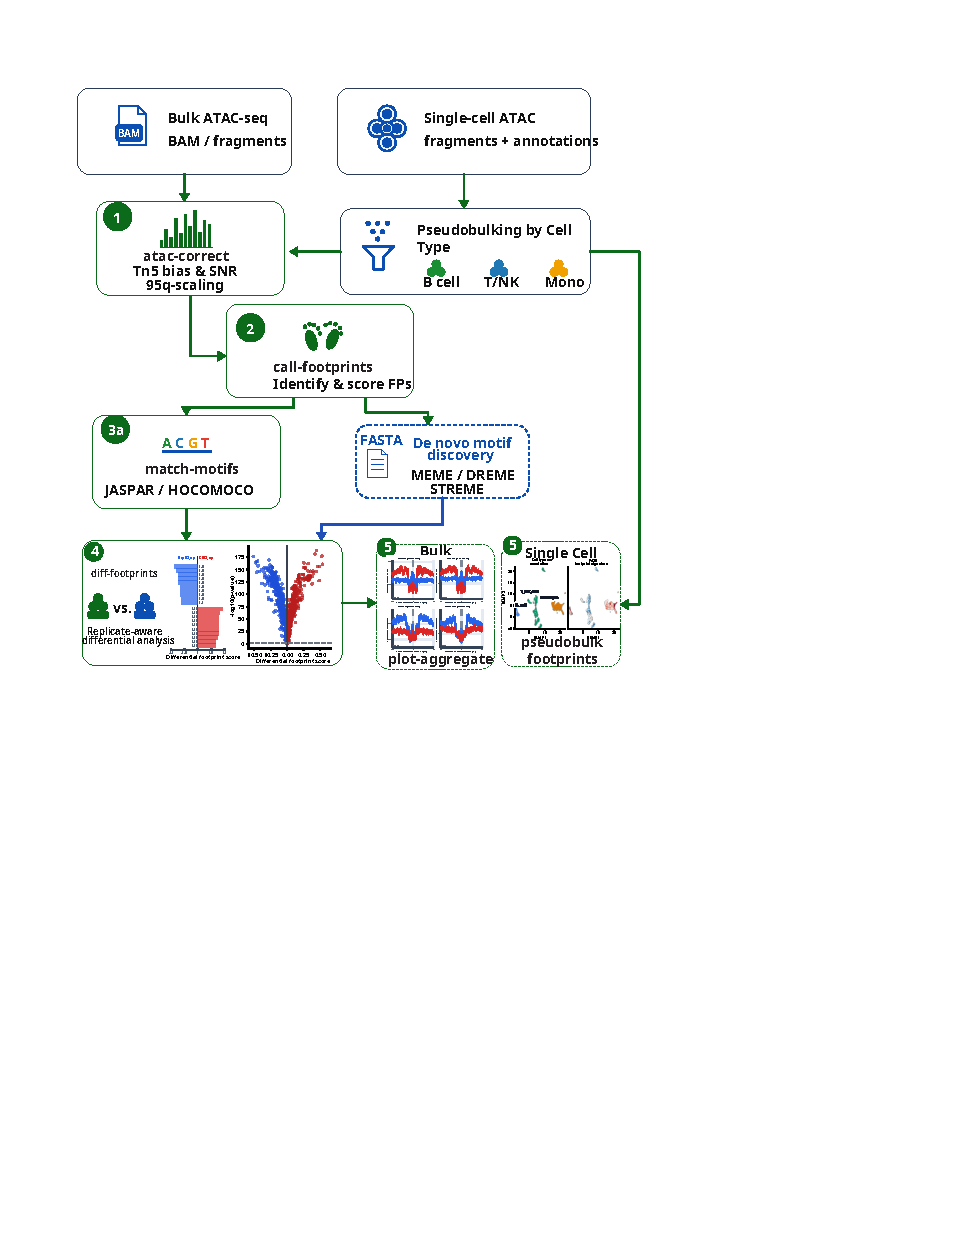
\includegraphics[height=0.56\textheight,keepaspectratio]{figures/Fig1.pdf}
\caption{Overview of the \texttt{fp-tools} ATAC-seq footprinting platform.
Bulk ATAC-seq BAM/fragments and single-cell ATAC fragments with annotations enter
a shared command-oriented analysis. The analysis supports Tn5 bias correction,
footprint calling, motif matching against curated databases, de novo motif
discovery, replicate-aware differential footprint analysis, aggregate footprint
visualization, and pseudobulk single-cell footprint analysis.
\label{fig:workflow_overview}}
\end{figure}


\subsection{De Novo Motif Discovery Complements Database-based Motif Analysis}

The de novo motif discovery path converts candidate footprint intervals into
centered FASTA files, runs MEME, DREME, or STREME, optionally compares discovered
motifs with a known database using Tomtom, and writes TSV/HTML summaries with
inline consensus logos. This extends the TOBIAS-style known-motif path by adding
a recorded handoff from footprint candidates to motif discovery; it does not
change the center-versus-flank footprint scoring model. The module can be run
alone to discover recurring sequence patterns in candidate intervals, or after
known-motif scanning to identify motifs that are absent from the selected
database.

We used public ENCODE K562 and HepG2 ATAC-seq data as two examples to evaluate
whether candidate footprint intervals contain recurring sequence motifs beyond a
curated database.
Candidate footprints were called from bias-corrected cut-site tracks, candidate
FASTA files were exported with 75 bp flanks, and reciprocal STREME runs were
performed using one cell line as the enriched sequence set and the other as the
sequence-control set. Discovered motifs were then summarized, compared with
JASPAR by Tomtom, and scanned back into candidate intervals for aggregate
footprint review.

The known-motif scan used JASPAR 2026 vertebrate non-redundant motifs, and
reciprocal STREME runs contributed candidate-derived motifs from both ENCODE cell
lines. Figure~\ref{fig:denovo_validation}B summarizes the merged de novo
motif-supported windows as either shared with the JASPAR-supported scan or
detected only by the de novo scan. The shared component dominated both K562 and
HepG2, while de novo-only windows accounted for 6.0\% of the total
de novo-supported merged window base pairs.

Representative discovered motifs showed clear motif-centered aggregate
footprint profiles in K562 and HepG2 (Figure~\ref{fig:denovo_validation}C,D),
indicating that the de novo sequence patterns correspond to footprinted cut-site
structure in the candidate intervals. Together with the recorded FASTA export,
motif discovery, and motif-comparison workflow
(Figure~\ref{fig:denovo_validation}A), these results support using de novo
motif discovery as a complement to database-based motif matching when the chosen
motif collection is incomplete or conservative.

\begin{figure}[!htb]
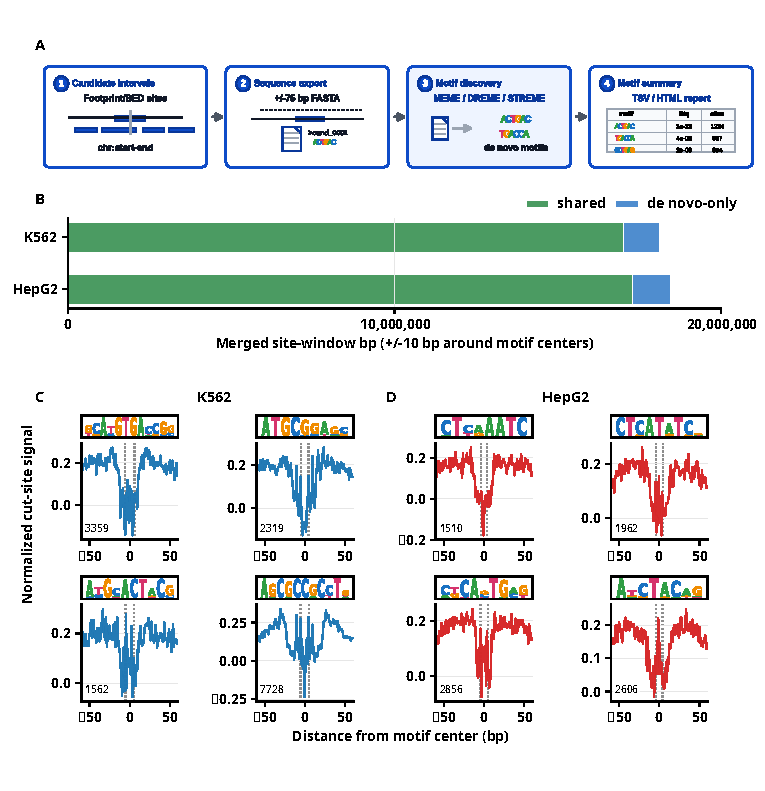
\includegraphics[width=\textwidth]{figures/Fig2.pdf}
\caption{De novo motif discovery and validation summary.
(\textbf{A}) Candidate footprint or BED intervals are converted into centered
FASTA sequences, analyzed with MEME/DREME/STREME, and summarized as motif tables
and reports. (\textbf{B}) Merged site-window coverage compares shared and
de novo-only motif-supported intervals in K562 and HepG2. (\textbf{C,D})
Representative K562 and HepG2 de novo motifs show footprint-like normalized
cut-site aggregate profiles centered on motif instances.
\label{fig:denovo_validation}}
\end{figure}

\subsection{Replicate-aware Differential Footprint Analysis}

We next evaluated replicate-aware differential footprint analysis using a 3-vs-3
public ENCODE ATAC-seq comparison between K562 and HepG2. All six replicates
were scanned on the same merged peak and motif-site universe before comparison,
so condition summaries, replicate-level variation, and motif rankings were
reported in a common coordinate framework.

A representative K562 versus HepG2 differential footprint report is shown in
Figure~\ref{fig:differential_report}. In this 3-vs-3 comparison, the report
ranked HNF4A, ONECUT2, and HNF4G motifs among the HepG2-biased signatures and
GATA2, TRPS1, and SP9 motifs among the K562-biased signatures. The bar plot and
volcano panel show the same directional separation, with HepG2-biased motifs on
the negative side of the differential footprint-score axis and K562-biased
motifs on the positive side. The replicate-level aggregate profiles provide a
second check on these rankings: for each selected motif, the three K562 and
three HepG2 traces are displayed separately, making replicate consistency and
motif-centered cut-site structure visible in the same report.

\begin{figure}[p]
\centering
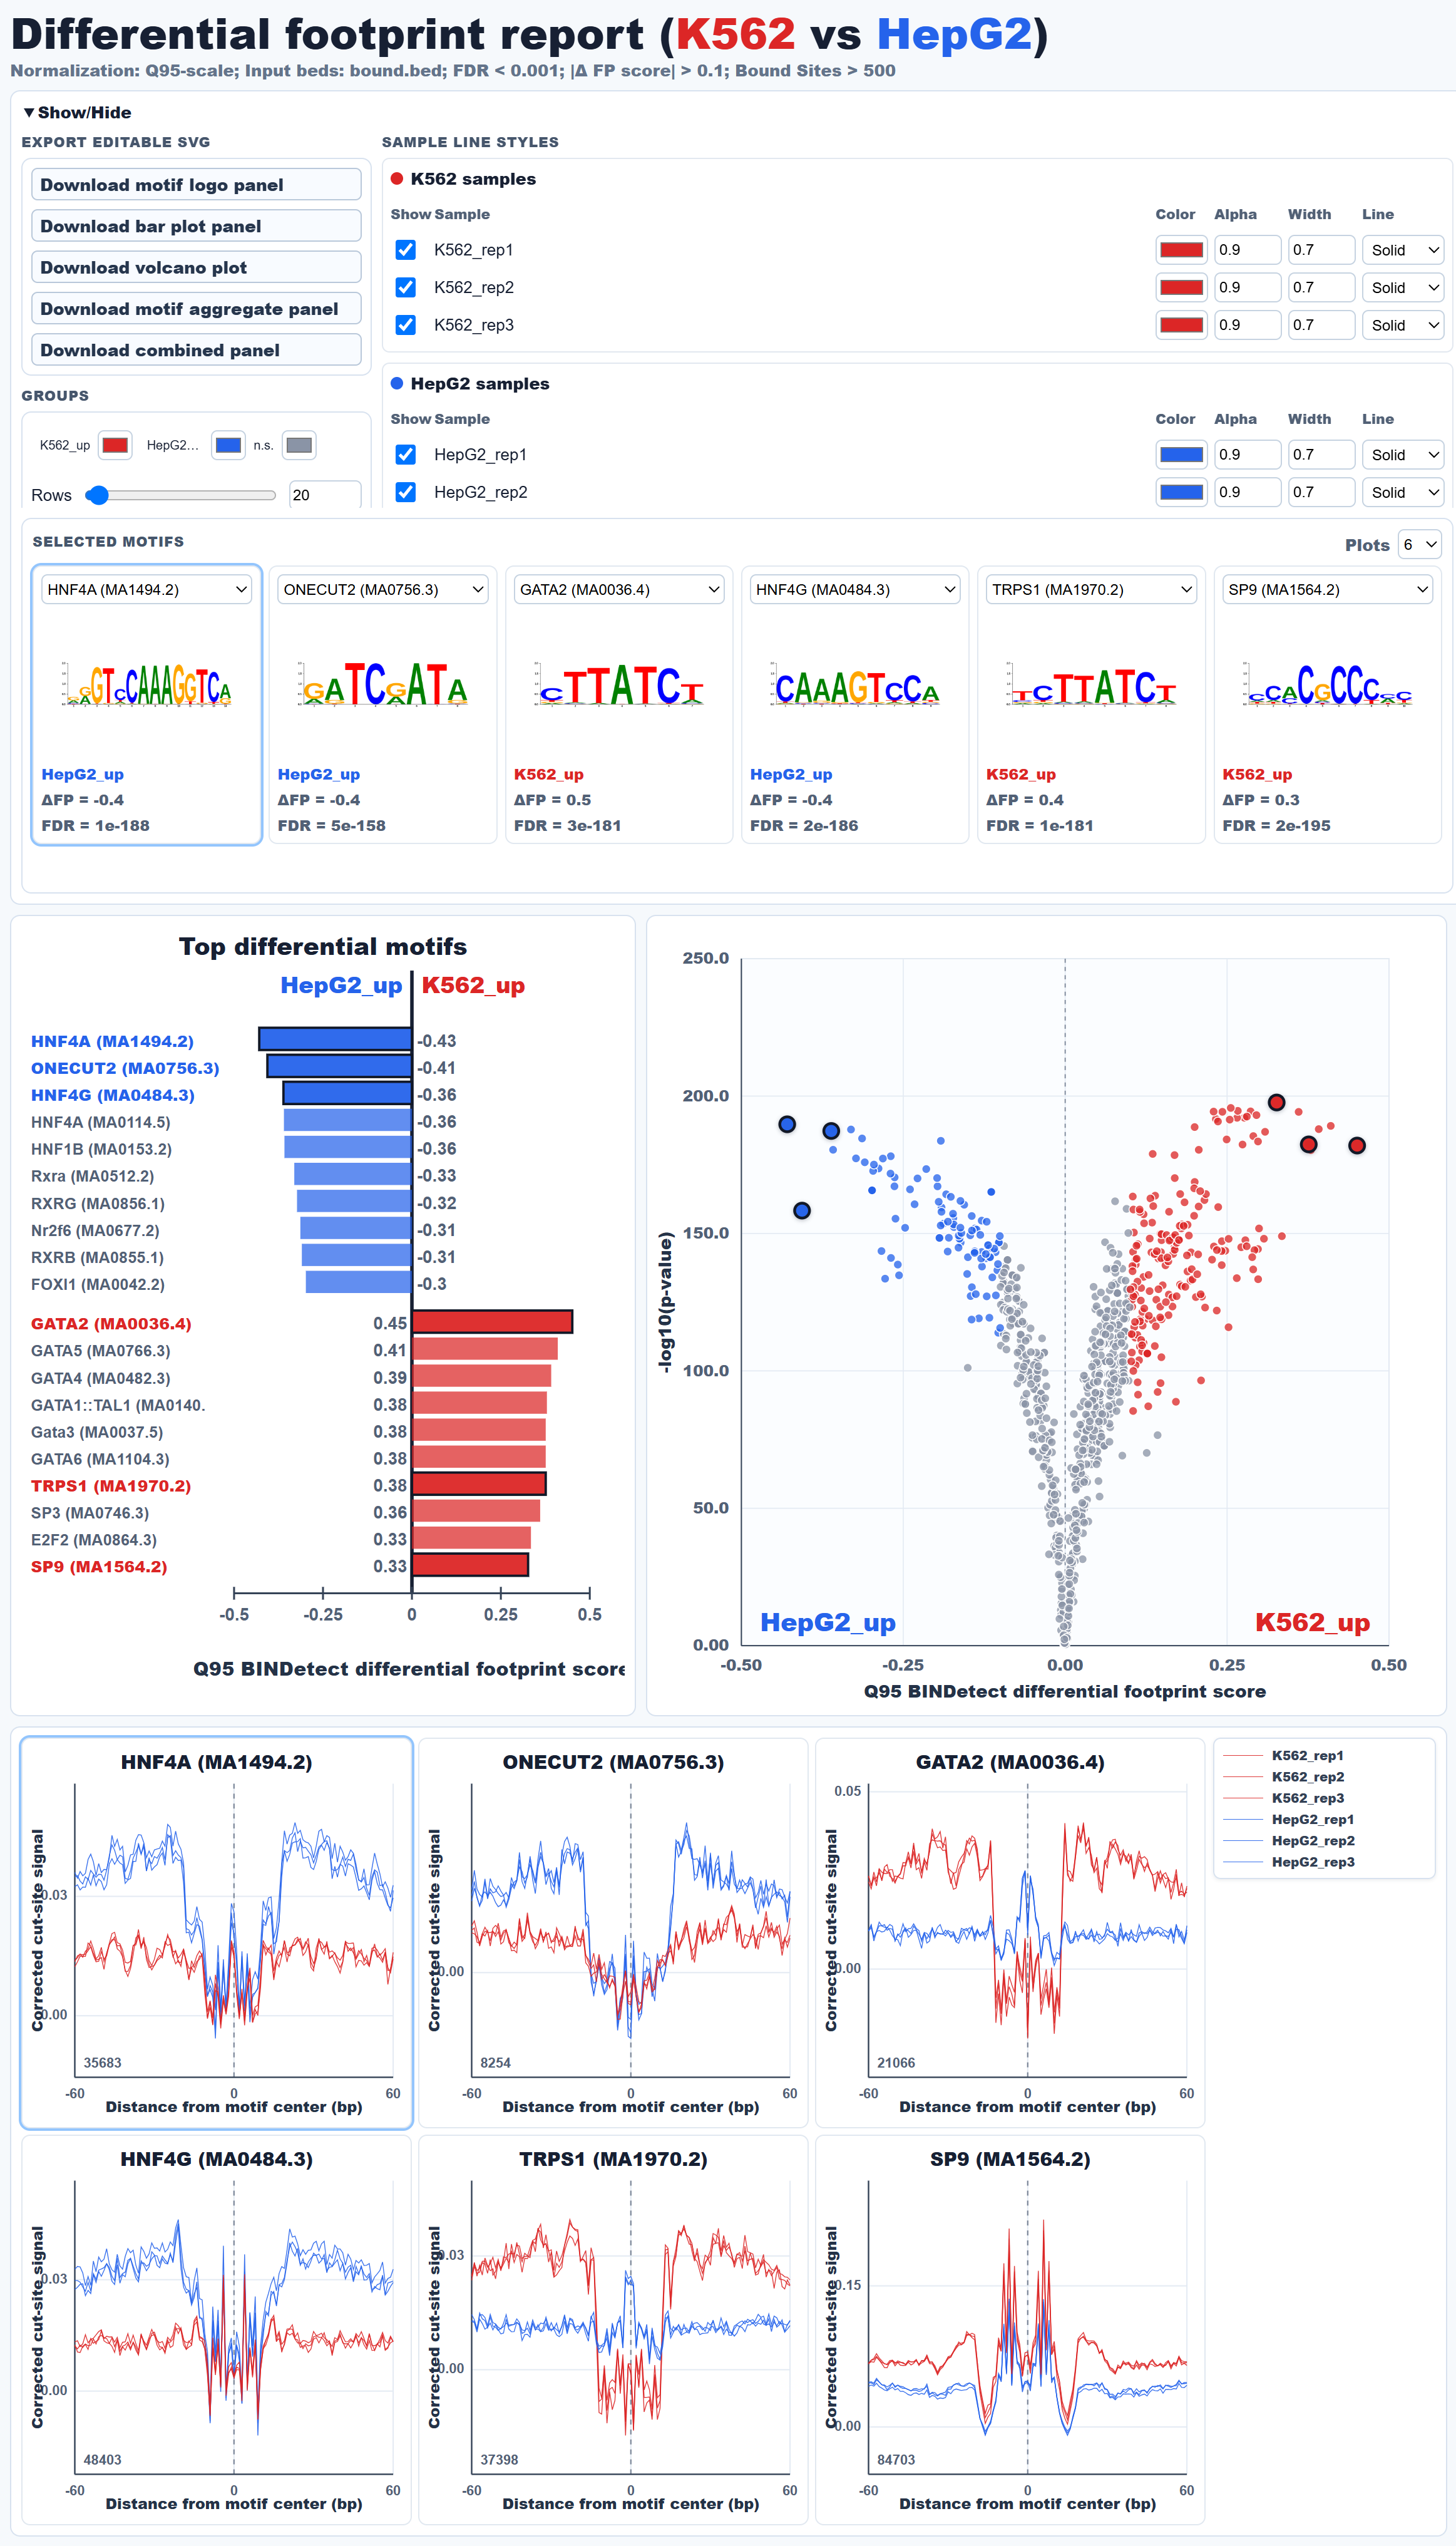
\includegraphics[height=0.88\textheight,keepaspectratio]{figures/Fig3.png}
\caption{Interactive differential footprint report for K562 versus HepG2.
The report summarizes selected differential motifs, motif logos, top
differential footprint-score bar plots, a volcano plot, and
replicate-level motif-centered aggregate profiles. Blue indicates HepG2-biased
footprint scores and red indicates K562-biased footprint scores.
\label{fig:differential_report}}
\end{figure}

\subsection{Single-cell ATAC Fragments Support Pseudobulk Footprinting}

We evaluated pseudobulk aggregation using the public 10x Genomics 5k PBMC
single-cell ATAC dataset~\cite{tenxpbmc5katac2021}. The demonstration used the
Cell Ranger ATAC 2.0.0 fragment file for \texttt{atac\_pbmc\_5k\_nextgem} and
broad cell annotations from the PBMC5k single-cell embedding. After filtering,
4,437 annotated cells were grouped into B cells (422 cells), monocytes (1,702
cells), and T/NK cells (2,313 cells). All three groups passed the pseudobulk
filters and contained 2.1, 10.8, and 13.3 million counted fragments,
respectively.

The marker-by-cell heatmap in Figure~\ref{fig:single_cell_footprinting}A shows
that KNN-smoothed footprint-signature scores separate the three broad PBMC
groups. B-cell-associated rows include STAT6 and FOSB; monocyte-associated rows
include CEBPA, IRF8, and RELA; and T/NK-associated rows include ZNF683, NR4A1,
and SMAD3. These row-level patterns show that motif-centered footprint
signatures derived from grouped single-cell fragments remain visible at the
cell-label level.

The UMAP panels in Figure~\ref{fig:single_cell_footprinting}B show the same
regulatory programs in the single-cell embedding. The broad-cell reference panel
separates B cells, monocytes, and T/NK cells. STAT6 and FOSB localize primarily
to the B-cell region, consistent with IL-4-responsive and AP-1-associated
activation programs. CEBPA, IRF8, and RELA localize to the monocyte region,
consistent with myeloid differentiation, interferon-regulatory, and
NF-\(\kappa\)B inflammatory programs. ZNF683, NR4A1, and SMAD3 localize within
the T/NK region, consistent with cytotoxic or resident-like, TCR-response or
tolerance-like, and TGF-\(\beta\)-associated regulatory-state programs.

\begin{figure}[!htb]
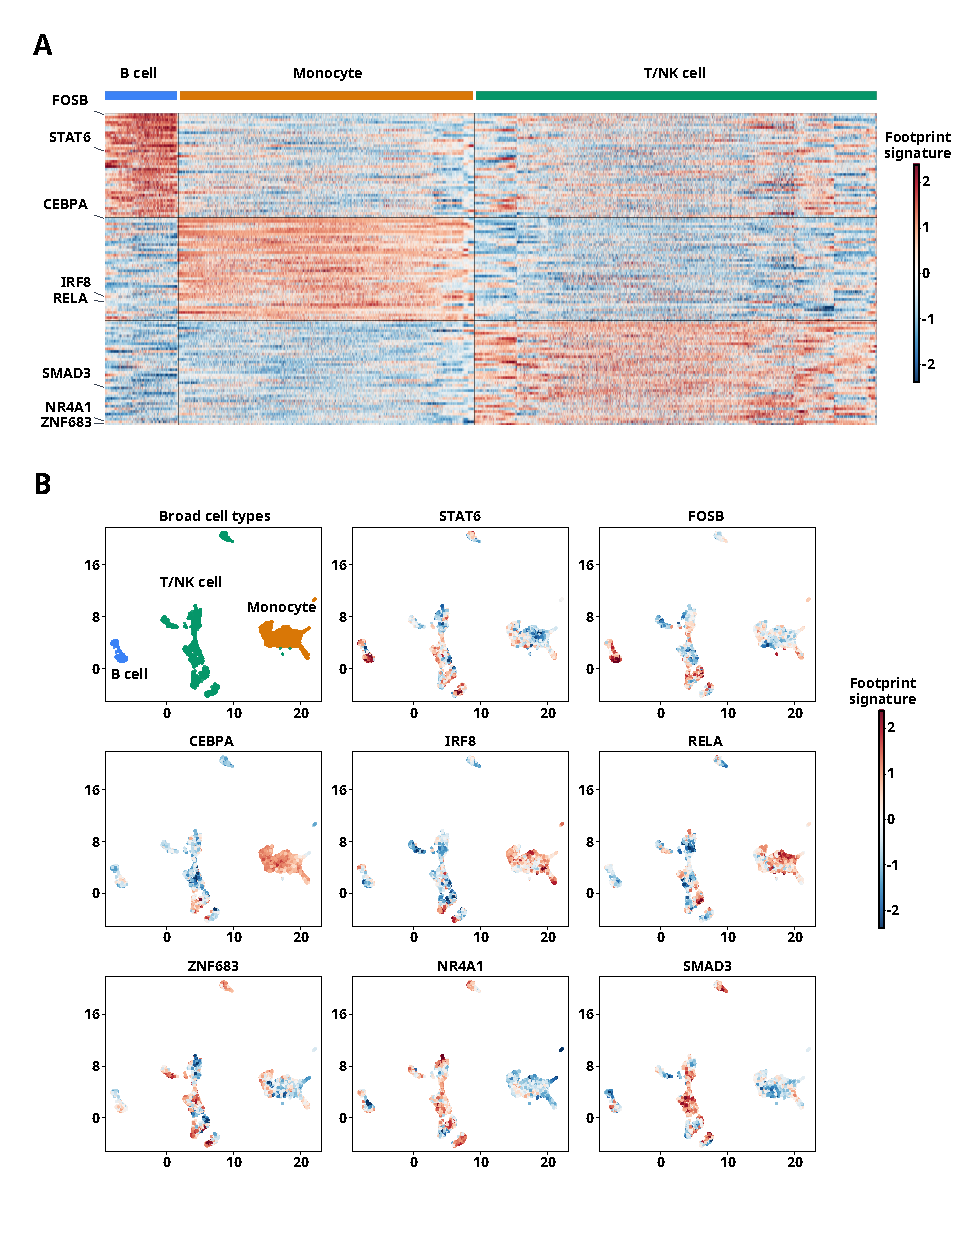
\includegraphics[width=\textwidth]{figures/Fig4.pdf}
\caption{Single-cell footprinting summary in public PBMC5k single-cell ATAC data.
(\textbf{A}) KNN-smoothed per-cell footprint-signature heatmap for top
cell-type-specific motif signatures across B cells, monocytes, and
T/NK cells;
the TF rows used for Panel B are labelled on the left. (\textbf{B}) UMAP
projections show broad cell-type annotations and representative motif-associated
footprint-signature z-scores. B-cell-associated signatures include STAT6,
consistent with IL-4-responsive humoral and class-switch-related signaling, and
FOSB/AP-1, consistent with an activation-responsive immediate-early regulatory
program. Monocyte-associated signatures include CEBPA, consistent with a
C/EBP-family myeloid differentiation program; IRF8, consistent with
monocyte/dendritic-cell and interferon-regulatory activity; and RELA, consistent
with NF-\(\kappa\)B-mediated inflammatory activation. T/NK-associated
regulatory-state signatures include ZNF683/Hobit, consistent with a cytotoxic or
resident-like program; NR4A1/Nur77, consistent with TCR-response and
tolerance-like regulation; and SMAD3, consistent with TGF-\(\beta\) regulatory
signaling. TF labels indicate motif-associated footprint signatures rather than
direct TF-specific occupancy.
\label{fig:single_cell_footprinting}}
\end{figure}

\subsection{Workflow Reproducibility, Benchmarking, and GUI Access}

The manuscript analyses are reproducible from public input manifests, recorded
command settings, and figure-generation scripts. Each analysis writes the
resolved input files, software versions, parameters, and plotting tables beside
the generated outputs. These records connect the bulk, de novo, pseudobulk,
replicate-aware, and report examples back to the exact sample, motif, region, and
signal-track choices used for each figure.

The package includes automated checks that run core commands on compact
reference inputs and compare key summary outputs for footprint calling,
differential footprint analysis, and aggregate plotting. Additional checks
exercise public command-line entry points and saved YAML configurations. These
tests help ensure that updates preserve expected workflow behavior and shared
input/output conventions.

We also benchmarked runtime and peak memory for the example workflow using the
same input bundle and matched command outputs for TOBIAS and \texttt{fp-tools}.
\texttt{fp-tools} completed the evaluated workflow in 16.7 min, compared with
30.3 min for TOBIAS (Figure~\ref{fig:engineering}A), and reduced peak memory
from 4.8 GB to 2.7 GB (Figure~\ref{fig:engineering}B). These measurements
support improved practical efficiency on the evaluated example dataset, while
remaining a single-machine benchmark rather than an exhaustive cross-tool
performance study.

\begin{figure}[!htb]
\centering
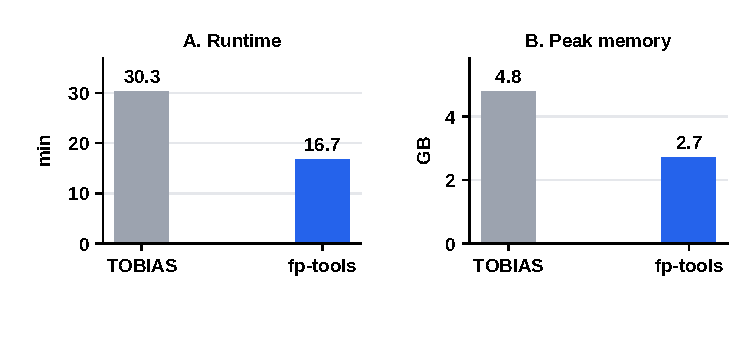
\includegraphics[width=0.50\textwidth]{figures/Fig5.pdf}
\caption{Single-machine runtime and memory benchmark.
(\textbf{A}) Runtime and (\textbf{B}) peak memory are summarized for one local
analysis run comparing TOBIAS and \texttt{fp-tools} on the same analysis bundle.
Lower values indicate faster execution and lower memory use.
\label{fig:engineering}}
\end{figure}

In addition to command-line execution, \texttt{fp-tools} provides a browser GUI
for configuring and running complete footprinting workflows. The GUI exposes the
major commands in the sidebar, including \texttt{atac-correct},
\texttt{call-footprints}, \texttt{match-motifs}, \texttt{diff-footprints},
aggregate plotting, and pseudobulk single-cell ATAC workflows. Users can choose
a command, load an example, fill in input paths and parameters, review the YAML
configuration, launch the run, and then inspect logs, tables, bigWigs, and HTML
reports from the run history (Figure~\ref{fig:gui_interface}). This design
allows users to complete the same analyses without writing command lines, while
the saved YAML configuration remains available for reruns and batch execution.

\begin{figure}[!htb]
\centering
\includegraphics[width=\textwidth,height=0.72\textheight,keepaspectratio]{figures/Fig6.png}
\caption{Browser GUI for complete footprinting workflows.
The GUI provides sidebar access to core bulk ATAC, report, and pseudobulk
commands; guided configuration panels; example loading; YAML preview; run
history; and direct review of logs, tables, bigWigs, and HTML reports.
\label{fig:gui_interface}}
\end{figure}

%==================================================================
\section{Discussion}
%==================================================================

\texttt{fp-tools} was developed to make motif-centered ATAC-seq footprinting
more reproducible, inspectable, and accessible without changing the core
biological interpretation of bias-corrected center-versus-flank footprint
signals. Rather than treating bias correction, motif scanning, differential
analysis, de novo motif discovery, pseudobulk aggregation, and report generation
as separate handoffs, \texttt{fp-tools} organizes them as one
command-compatible workflow (Table~\ref{tab:features}). This design is useful
because footprinting analyses often depend on small but important choices in
region definitions, motif sets, sample labels, signal scaling, and plotting
inputs. Keeping these choices in one recorded workflow makes the analysis easier
to review and reproduce.

TOBIAS remains the closest methodological reference point, because it established
a widely used and interpretable workflow for ATAC-seq bias correction, footprint
scoring, motif-aware differential analysis, and aggregate visualization.
\texttt{fp-tools} builds on this signal model while adding reusable YAML
configurations, de novo motif discovery with database matching,
replicate-aware reporting, pseudobulk single-cell footprinting, interactive
HTML/SVG outputs, a browser GUI, and tested public-data examples. These additions
are intended to lower practical barriers for users who need a workflow that can
be run from the command line, reviewed in a browser, reproduced from saved
configuration files, and traced from public inputs to final figures.

\begin{table}[H]
\caption{Qualitative scope comparison of ATAC-seq regulatory-analysis tools.
\checkmark, native support; $\circ$, partial or adjacent support; NA, outside
the tool's main scope. This table summarizes documented features, not benchmark
performance.
\label{tab:features}}
\begingroup
\footnotesize
\setlength{\tabcolsep}{2pt}
\renewcommand{\arraystretch}{1.06}
\newcommand{\featureyes}{\checkmark}
\newcommand{\featurepartial}{$\circ$}
\begin{tabularx}{\textwidth}{>{\raggedright\arraybackslash}p{0.30\textwidth}*{6}{>{\centering\arraybackslash}p{0.085\textwidth}}}
\toprule
\textbf{Feature} & \textbf{fp-tools} & \textbf{TOBIAS} & \textbf{\shortstack{HINT-\\ATAC}} & \textbf{\shortstack{PRINT/\\scPrinter}} & \textbf{\shortstack{Chrom\\BPNet}} & \textbf{\shortstack{max\\ATAC}}\\
\midrule
Bulk ATAC footprinting & \featureyes & \featureyes & \featureyes & \featureyes & \featurepartial & NA\\
Tn5 bias correction & \featureyes & \featureyes & \featureyes & \featureyes & \featureyes & NA\\
Footprint calling & \featureyes & \featureyes & \featureyes & \featureyes & NA & NA\\
Motif-aware differential analysis & \featureyes & \featureyes & \featurepartial & \featurepartial & NA & NA\\
De novo motif discovery & \featureyes & NA & NA & \featureyes & \featurepartial & NA\\
scATAC/pseudobulk support & \featureyes & \featurepartial & \featurepartial & \featureyes & \featurepartial & \featurepartial\\
Replicate-aware reporting & \featureyes & \featurepartial & \featurepartial & \featurepartial & NA & NA\\
Visualization/reporting & \featureyes & \featureyes & \featurepartial & \featureyes & \featureyes & \featurepartial\\
YAML/batch execution & \featureyes & NA & NA & NA & NA & NA\\
\bottomrule
\end{tabularx}
\let\featureyes\undefined
\let\featurepartial\undefined
\endgroup
\end{table}

The public examples illustrate how these additions extend routine footprint
analysis. In the ENCODE bulk ATAC-seq examples, de novo motif discovery
recovered candidate-derived sequence patterns that produced motif-centered
aggregate footprint profiles and overlapped substantially with JASPAR-supported
bound-site windows. In the K562/HepG2 replicate comparison, the report combined
native motif-background footprint summaries with replicate-supported motif-score
statistics and replicate-level aggregate profiles. In the PBMC5k single-cell
example, pseudobulk aggregation produced bulk-like inputs for corrected
footprint tracks, whereas KNN-smoothed cell-level signatures provided a
visualization of cell-type-associated motif-centered cut-site patterns on the
UMAP.

These use cases also clarify the intended scope of the package. Deep
sequence-to-profile models such as ChromBPNet learn sequence determinants of
chromatin profiles and are well suited for occupancy and variant-effect
analyses~\cite{chrombpnet2024}. Accessibility-based frameworks such as diffTF
estimate differential TF activity from changes in open chromatin rather than
from motif-centered footprint profiles~\cite{Berest2019_diffTF}. Single-cell
packages such as ArchR and Signac provide broad ecosystems for single-cell
chromatin analysis, while chromVAR provides a widely used baseline for
motif-deviation analysis. These approaches are complementary to motif-centered
footprinting rather than direct replacements. In this landscape,
\texttt{fp-tools} is intended as an auditable route from ATAC-seq cut-site signal
to motif-level footprint interpretation.

Several limitations remain. The runtime and memory benchmark was performed on
the defined example workflow and demonstrates the efficiency gains in that
setting; additional datasets and hardware environments will help quantify
scaling across broader use cases. The de novo motif analysis provides
operational motif-window recovery summaries rather than formal differential
binding significance tests. The cell-level footprint signatures are KNN-smoothed
visual summaries of local motif-centered cut-site patterns and should not be
interpreted as direct TF-specific occupancy calls in individual cells. Future
work will therefore focus on larger controlled benchmarks, broader biological
validation, and additional replicate designs across tissues, perturbations, and
sequencing depths.

%==================================================================
\section{Conclusions}
%==================================================================

We presented \texttt{fp-tools} as a Python platform for reproducible,
user-accessible ATAC-seq footprint analysis across bulk and single-cell-derived
pseudobulk data. The package combines command-line execution, reusable YAML
configuration, de novo motif discovery, replicate-aware reporting, pseudobulk
footprinting, interactive reports, and a browser GUI in a single workflow.
Across public bulk and single-cell examples, \texttt{fp-tools} preserved the
core interpretation of bias-corrected center-versus-flank footprints while
extending the workflow to motif discovery, replicate-supported review, and
single-cell pseudobulk analysis.

\vspace{6pt}

\authorcontributions{Conceptualization, Y.L. and C.Y.; methodology, Y.L.; software,
Y.L.; validation, Y.L.; formal analysis, Y.L.; investigation, Y.L.; data curation,
Y.L.; writing, original draft preparation, Y.L.; writing, review and editing, Y.L.
and C.Y.; visualization, Y.L.; supervision, C.Y.; project administration, C.Y.;
funding acquisition, C.Y. All authors have read and agreed to the published version
of the manuscript.}

\funding{This research received no external funding.}

\institutionalreview{Not applicable. This study used only publicly available,
de-identified datasets and did not involve new experiments on humans or animals.}

\informedconsent{Not applicable.}

\dataavailability{\texttt{fp-tools} is openly available in the public GitHub
repository \href{https://github.com/oncologylab/fp-tools}{\mbox{\texttt{oncologylab/fp-tools}}}.
The repository contains the manifests, schemas, analysis scripts, figure
generators, source tables, and small result tables used in this manuscript.
Public input data are obtained
from the ENCODE Project~\cite{encode2012}, the 10x Genomics PBMC5k single-cell
ATAC example~\cite{tenxpbmc5katac2021}, and motif databases such as
JASPAR~\cite{jaspar2026} using the included download and preparation scripts.
The computational environment is documented in \texttt{environment.yml} and the
repository Dockerfile.}

\acknowledgments{The authors thank the ENCODE Project Consortium and the
maintainers of the open-source tools referenced in this work for making their data
and software publicly available.}

\conflictsofinterest{The authors declare no conflicts of interest.}


%==================================================================
\appendix
\section*{Appendix}
\renewcommand{\thetable}{S\arabic{table}}
\setcounter{table}{0}
%==================================================================

\begin{table}[H]
\caption{Primary analysis parameters used for the public ATAC and pseudobulk workflows. The complete source table is provided in the Supplementary Materials as ``Primary analysis parameters''.\label{tab:supp_analysis_parameters}}
\begingroup
\scriptsize
\renewcommand{\arraystretch}{1.04}
\begin{tabularx}{\textwidth}{>{\bfseries\raggedright\arraybackslash}p{0.26\textwidth}>{\raggedright\arraybackslash}X}
\toprule
\textbf{Step} & \textbf{Parameters}\\
\midrule
Public input data & Bulk ATAC analyses use public ENCODE K562/HepG2 replicate BAMs and tracks. The pseudobulk single-cell demonstration uses the public 10x Genomics 5k PBMC scATAC fragment dataset. Motif analyses use JASPAR 2026 CORE vertebrate non-redundant motifs.\\
ENCODE BAM processing & Released GRCh38 alignment BAMs for K562 ENCSR868FGK and HepG2 ENCSR291GJU were filtered to standard chromosomes, indexed, and summarized before footprint analysis.\\
Blacklist and peak set & Mitochondrial and nonstandard contigs excluded; hg38 blacklist v2 regions subtracted; released ENCODE peak intervals sorted and merged across replicates into one analysis peak set.\\
Bias correction and footprint scores & \texttt{atac-correct} run on filtered BAMs with merged peaks and blacklist regions using default Tn5-bias settings; corrected cut-site tracks q95-scaled over shared background regions for multi-sample analyses; \texttt{call-footprints --score footprint} run with default footprint and flank windows.\\
Differential footprint analysis & The 3-vs-3 ENCODE K562/HepG2 replicate footprint tracks were analyzed with repeated condition labels, JASPAR 2026 motifs, and replicate reporting enabled. Single-sample contrasts use motif-site versus background-distribution comparison; replicate-supported analyses use empirical-Bayes variance moderation on per-sample aggregated motif scores.\\
De novo motif validation & ENCODE K562/HepG2 candidate footprints exported as cell-line-level FASTA files with \(\pm 75\) bp flanks; reciprocal STREME 5.5.9 runs used \texttt{--dna --nmotifs 250}; Tomtom 5.5.9 matched discovered motifs to JASPAR 2026; discovered motifs were scanned back into candidate intervals for motif-window overlap summaries and aggregate footprint review.\\
Pseudobulk PBMC analysis & Public 10x PBMC5k scATAC fragments grouped into broad B-cell, monocyte, and T--NK labels, retaining 4,437 annotated cells and requiring at least 300 cells and 50,000 fragments per group. The full \texttt{pseudobulk-footprints} route writes pseudo-BAMs, runs ATAC correction with zero read shifting for fragment-derived pseudobulk BAMs, and emits footprint-score tracks, motif-aware differential results, marker heatmaps, and KNN-smoothed footprint-signature UMAPs.\\
\bottomrule
\end{tabularx}
\endgroup
\end{table}

\begin{table}[H]
\caption{Software and resource versions used for manuscript analyses. The complete source table is provided in the Supplementary Materials as ``Software and resource versions''.\label{tab:supp_software_versions}}
\begingroup
\footnotesize
\renewcommand{\arraystretch}{1.04}
\begin{tabularx}{\textwidth}{>{\raggedright\arraybackslash}p{0.28\textwidth}>{\raggedright\arraybackslash}p{0.14\textwidth}>{\raggedright\arraybackslash}X}
\toprule
\textbf{Tool or resource} & \textbf{Version} & \textbf{Role}\\
\midrule
\texttt{bedtools} & 2.31.1 & Region sorting, merging, and blacklist subtraction\\
Biopython & 1.87 & Sequence and motif-related utilities\\
Cell Ranger ATAC & 2.0.0 & Source processing for the public 10x PBMC5k scATAC dataset\\
\texttt{fp-tools} & 0.1.7 & ATAC correction, footprint calling, motif matching, differential footprint analysis, pseudobulk utilities, and plotting helpers\\
hg38 blacklist & v2 & Artifact-region filtering for processed bulk ATAC alignments\\
hg38 reference genome & GRCh38/hg38 & Sequence extraction and ATAC bias correction\\
htslib & 1.23.1 & SAM/BAM/VCF I/O backend used by \texttt{samtools}\\
JASPAR CORE vertebrates & 2026 non-redundant & Known motif database for differential footprint analysis\\
matplotlib & 3.10.9 & Manuscript figure rendering\\
MEME Suite, STREME, and Tomtom & 5.5.9 & De novo motif discovery and discovered-motif matching\\
NumPy & 2.4.6 & Numerical arrays and benchmark/figure calculations\\
pandas & 2.3.3 & Tabular processing for benchmark, manifest, and figure builders\\
pyBigWig & 0.3.25 & bigWig signal reading and writing\\
pysam & 0.23.3 & BAM and genomic interval I/O\\
Python & 3.12.3 & Runtime for analyses, figure builders, and provenance extraction\\
\texttt{samtools} & 1.23.1 & Released ENCODE BAM filtering, indexing, and QC summaries\\
SciPy & 1.17.1 & Statistical and interpolation utilities\\
\bottomrule
\end{tabularx}
\endgroup
\end{table}

%==================================================================
\bibliography{references}

\end{document}
